\RequirePackage[hyphens]{url}
\documentclass[sigconf]{acmart}
%\raggedbottom
%\sloppy

\usepackage{hyperref}

%\usepackage{endfloat}
%\renewcommand{\efloatseparator}{\mbox{}} % no new page between figures

\usepackage{booktabs} % For formal tables

\settopmatter{printacmref=false} % Removes citation information below abstract
\renewcommand\footnotetextcopyrightpermission[1]{} % removes footnote with conference information in first column
\pagestyle{plain} % removes running headers


\begin{document}

\title{BigchainDB: A Big Database for the Blockchain?}
\author{Timothy A. Thompson}
%\orcid{0000-0001-6574-9010}
\affiliation{%
  \institution{Indiana University Bloomington}
  \streetaddress{School of Informatics, Computing, and Engineering}
  \city{Bloomington} 
  \state{Indiana} 
  \postcode{47408}
}
\email{timathom@indiana.edu}

\begin{abstract} 
Decentralized systems such as Bitcoin, the Interplanetary File System, and Ethereum have been designed with the intention of reengineering the architecture of online information networks, of minimizing exposure caused by central points of failure, and of creating new social models for the exchange of data---which is posited as a valuable asset in and of itself. Are these kinds of systems also able to support big data analytics and processing? If so, what stands to be gained by taking a blockchain-based approach to big data? Efforts to integrate blockchains into big data pipelines must inevitably address the tradeoff between security and scalability. BigchainDB is a new decentralized database framework that adds blockchain-based features, such as immutability and secure asset management, to traditional NoSQL distributed databases. Although it is still in the early stages of development, BigchainDB promises to make a significant contribution to the ways in which data is shared, processed, and managed at scale.
\end{abstract}

\keywords{i523, HID340, Decentralization, Databases, NoSQL, Blockchains, BigchainDB}

\maketitle

\section{Introduction}
Approaches to managing and processing big and complex data, such as the Lambda Architecture framework, have stressed the importance of treating data as an immutable asset \cite{nM15}. In this view, data should never be updated, but only appended. In systems that allow data to be deleted or updated, big data only amplifies the surface of exposure to human error, and systems that conform to the standard relational database model of incremental updates become increasingly brittle as the scale of data increases \cite{nM15}. Inadvertent deletions can trigger a cascade of data loss and system disruption that can be particularly difficult and costly to recover from. Even those who have criticized the specifics of the Lambda Architecture model (which proposes a complex internal division, within big data systems, between a batch layer and a realtime layer) agree that data immutability is an important foundation for building massively scalable platforms \cite{jK14}.

In decentralized, blockchain-based systems such as Bitcoin, immutability takes on an even more critical role. Without immutability and concomitant mechanisms such as Merkle tree hashing, it would not be possible to verify Bitcoin transactions for authenticity, nor would it be possible to maintain the ``trustless'' nature of the network---which is what allows decentralization itself to succeed \cite{aA17}. In addition to Bitcoin, the emerging decentralized data ecosystem currently comprises platforms for computation (Ethereum) and file storage (Interplanetary File System---IPFS), but database software for managing metadata about assets is still lacking. BigchainDB is a databse solution that has been designed to fill this niche \cite{bigDB16, tMBI15}.

\section{Distributed versus Decentralized}
Once it has been elevated to a core piece of system architecture, data immutability can become either a burden or an opportunity. The Lambda Architecture model leverages immutability within the context of an internally distributed environment, using storage solutions such as the Hadoop Distributed File System (HDFS) for processing on the batch layer \cite{nM15}. Distributed systems are not the same as decentralized systems, however, and the terminology itself can be misleading, as illustrated by Baran's often-reproduced work depicting the continuum between centralized and distributed networks (shown in Figure \ref{f:baran}). In Baran's model, decentralized networks are vulnerable to attack because of their reliance on hubs, whereas distributed networks are more durable because they employ a resilient grid-like structure \cite{pB64}. In the context of the current discussion, ``decentralized'' systems such as Bitcoin are in fact exemplars of distributed models of connectivity. Distributed file systems such as HDFS, by contrast, may exist within highly centralized platforms or services. Here, the term decentralized will be used to refer to systems that embrace distributed models of organization both internally and externally. 

\begin{figure}
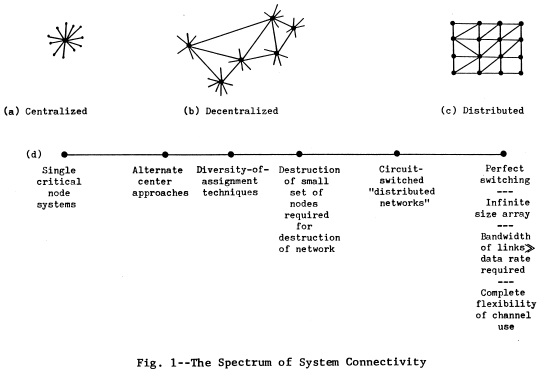
\includegraphics[width=1.0\columnwidth]{images/baran-fig1.png}
\caption{Baran's centralized--distributed network continuum \cite{pB64}}
\label{f:baran}
\end{figure}

\subsection{Tradeoffs between Security and Scalability}
Bitcoin's high level of security and resistance to attack are appealing features to engineers concerned with issues of data integrity. However, the Bitcoin network and blockchain are currently not equipped to manage big data \cite{kC16}. Compared to commercial financial transaction processors, which are capable of processing thousands of transactions per second, Bitcoin's computationally intensive ``Proof of Work'' model limits the network's throughput to a maximum of about 7 transactions per second \cite{kC16}. Recommendations for improving the scalability of distributed ledgers such as Bitcoin range from adjusting system parameters (for example, maximum block size) to sharding the transaction validation layer in order to take advantage of parallel processing; however, the need for community approval and adoption of scalability solutions means that changes will take time to be implemented \cite{kC16}.

\subsection{Blockchains for Big Data}
The Bitcoin blockchain could itself be viewed as a globally distributed database, albeit not a particularly efficient or effective one. What is the primary benefit, then, of attempting to bring blockchain-based technologies to bear on big data? The potential value of integrating blockchains into big data pipelines is extrinsic rather than intrinsic: blockchains do not enable new analytical frameworks or algorithms per se, but rather promise to revolutionize the economies of exchange that determine the value and availability of big data \cite{tMBD16}. Nevertheless, in order for big data pipelines to be ``blockchainified,'' the issue of scalability must still be addressed. Because a systematic reengineering of blockchain systems such as Bitcoin seems unlikely in the near term, an alternative approach would be to modify existing big data systems by wrapping them with a blockchain layer. The latter approach is the one that has been adopted by the designers of BigchainDB \cite{bigDB16}.

\section{BigchainDB}
BigchainDB is a database framework designed to extend the capabilities of existing NoSQL databases. To date, development of BigchainDB has focused on integration with two systems: RethinkDB (\url{https://www.rethinkdb.com/}) and MongoDB (\url{https://www.mongodb.com/}), although only the latter is recommended for usage as a production server \cite{bigDB17b}. Adding a blockchain layer to proven database systems allows developers to obviate or offload many of the problems with scalability and throughput currently faced by Bitcoin, for example. The BigchainDB whitepaper specifies three areas of innovation in which blockchain characteristics have been added as extensions to RethinkDB and MongoDB: decentralized control, immutability, and the creation and transfer of digital assets \cite{bigDB16}.

\subsection{Decentralized control}
A primary goal of BigchainDB's designers was to support seamless integration with the emerging ecosystem of ``trustless decentralization'' \cite{bigDB16}. In order for a trustless approach to be viable, solutions to traditional distributed database problems such as consensus (how are conflicts among database nodes resolved?) must be implemented. In this regard, the BigchainDB whitepaper discusses three areas of concern: benign faults, Byzantine faults, and Sybil attacks \cite{bigDB16}. To address benign faults (for instance, those caused by hardware failure), the default consensus protocol of the underlying database system is relied upon \citep{bigDB16}. Although no claims are made for full Byzantine fault tolerance, the whitepaper goes into considerable detail regarding mechanisms for voting on and validating distributed transactions. Finally, Sybil attacks (in which a bad actor perpetrates a hostile takeover of a network) are addressed on the level of governance: the whitepaper describes a scenario in which BigchainDB nodes are deployed in a ``federation with a high barrier of entry based on trust and reputation'' \citep{bigDB16}.

\subsection{Immutability}
Data stored in a BigchainDB instance is treated as immutable and validated through a standard blockchain procedure of cryptographic hashing. Once a transaction has been approved by a majority of database nodes and fully validated, it is added to the system's internal blockchain, where is no longer exposed for updating or deletion. The approach to data management adopted by BigchainDB is known as CRAB (Create, Retrieve, Append, Burn)---in contrast to the CRUD (Create, Read, Update, Delete) model of traditional relational database systems \cite{jP17}. Database assets that are ``burned'' are, in fact, not removed from persistent storage, but are simply reassigned to a randomly generated public key and effectively lost to the system \citep{jP17}.

\subsection{Digital asset creation and transfer}
At the core of BigchainDB is the framework that it provides for the secure transfer and tracking of assets in a chain of custody. Metadata surrogates can be created for both born-digital and real-world assets and assigned to individual users, identified by their public keys (from a system-generated public-private key pair). Assignment (that is, ownership) of metadata for assets can then be transferred from one user to another. The ability to make and authenticate claims about ownership is particularly valuable for content creators who wish to assert, and profit from, their intellectual property rights. Original development of BigchainDB was driven by the company ascribe.io, which provides artists with a platform for recording ``art attribution, transfer, consignment and loan records'' related to their work \cite{bigDB17a}.

\section{Conclusion}
As a big data management system, BigchainDB promises to make it possible to attach ``audit trails'' to datasets, adding to their value by confirming their trustworthiness and integrity \cite{tMBD16}. It also has the potential to serve as a decentralized clearinghouse for data sharing. Currently, access to data---including openly licensed data---is controlled by central service providers, in part to bolster assurances of the data's authenticity or accuracy. If data, instead, were stored in a decentralized blockchain database, it could be ``collectively controlled by a public ecosystem'' as an open marketplace \cite{tMBD16}. Concerns about competitive advantage would be minimized because all parties would have a stake in ensuring the success of this global data exchange, and none would have the ability to control it directly or attempt to exclude other stakeholders from the opportunity to participate and profit. 

Breaking down silos and providing incentives for data sharing also stand to benefit fields such as machine learning and artificial intelligence \cite{tMAI17}. One lesson of the big data revolution was that the accuracy of models could improve if enough data became available for analysis and training---and that simpler algorithms could often outperform more complex ones if the scale of data were large enough \cite{tMAI17}. New possibilities for sharing data through decentralized, secure systems could now make it possible to leverage the scale of big data on an even bigger scale \cite{tMAI17}.

\begin{acks}
The author would like to thank Dr. Gregor von Laszewski and the i523 teaching assistants for their support and suggestions in writing this paper.
\end{acks}

\bibliographystyle{ACM-Reference-Format}
\bibliography{report} 

\end{document}

























